% !TeX root = ../main.tex

\chapter{实验结果及分析}

\section{数据增广}

\subsection{输入数据的全局对齐问题}

当我们用手绘草图测试训练好的模型时,发现如下问题:当手绘草图的人脸特征点与参考底图基本重合时,生成效果非常不错;但是当我们手绘草图的位置偏离底图时,生成效果则非常糟糕。

由于CalebA-HQ数据集的人脸照片是以面部特征点为参照进行裁剪的,我们的训练数据——轮廓图也是基于面部特征点获取的,所以我们直觉地认为所有训练数据的特征点都具有空间一致性。

为证实以上假设,我们计算了所有训练数据的平均脸,如图~\ref{fig:average_face}~所示。我们发现其五官和面部轮廓基本处于相同位置,换句话说训练数据是全局对齐的。
\begin{figure}[htb]
	\centering
	\includegraphics[width=0.3 \textwidth]{average_face.png}
	\caption{轮廓图平均脸}
	\label{fig:average_face}
\end{figure}

这就导致了测试结果对输入数据空间分布变化包容性差的问题。使用者便只能被限制在固定的区域,不能随心所欲地在界面上不同位置绘制草图了。

\subsection{训练数据的增广}

我们通过对训练集的草图做一定程度的平移和旋转来模拟用户手绘草图空间位置的变化。平移在水平和竖直两个方向上进行,平移的距离在$\pm 25$像素之间随机选取,旋转的范围在$-7^{\circ} \sim +7^{\circ}$之间。但是人脸照片并不做平移和旋转处理,因为我们期望无论输入草图的空间位置如何,生成结果始终保持全局对齐。我们用增广后的数据重新训练模型。

用手绘草图对模型进行测试,发现对于不同方向产生位移的草图,使用增广数据训练后的模型的生成效果要明显优于原始模型,如图~\ref{fig:data_augmentation}。
\begin{figure}[htb]
	\centering
	\includegraphics[width=0.6 \textwidth]{data_augmentation.png}
	\caption{数据增广前后生成结果对比}
	\label{fig:data_augmentation}
\end{figure}

\section{我们模型的生成效果及对比实验}

\subsection{针对实例标准化的消融实验}

我们称原始的pix2pixHD的模型为$M_1$,在pix2pixHD的$G_1$基础上去掉前5层实例标准化的模型为$M_2$。用手绘的草图对我们的模型及以上2个模型分别进行测试,得到的结果如图~\ref{fig:ablation}~所示:
\begin{figure}[htb]
	\centering
	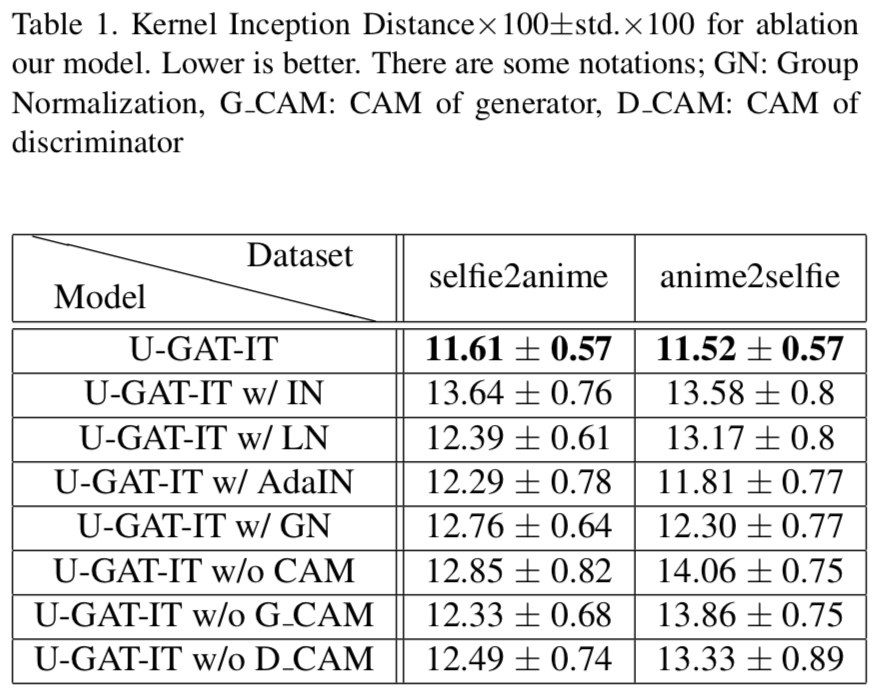
\includegraphics[width=0.8 \textwidth]{ablation.png}
	\caption{针对实例标准化层数量的对比实验}
	\label{fig:ablation}
\end{figure}

可以看到,我们模型的生成效果最好,图像的对比度更高,光照也更加自然,而$M_2$的生成结果会出现蓝绿等不正常色块,降低了人脸的真实感。这是因为$M_2$把生成器特征提取阶段的实例标准化操作都去掉之后,使最终提取出来的特征很多地方值为0,造成反向传播过程中梯度消失,训练过程很难收敛。

下面,只比较我们的模型与原模型pix2pixHD之间生成结果的差异。

\subsection{我们的模型与pix2pixHD的对比实验}

首先我们的细节更加逼真,纹理更加丰富。比如牙齿位置,pix2pixHD的结果产生模糊,而我们的结果则纹理清晰,细节丰富。再比如额头位置,pix2pixHD的生成结果经常出现一些乱发状的噪声,而我们的结果则没有这个问题,如图~\ref{fig:compare_1}~所示。
\begin{figure}[htb]
	\centering
	\includegraphics[width=0.65 \textwidth]{texture.png}
	\caption{我们的模型与pix2pixHD的生成结果细节对比}
	\label{fig:compare_1}
\end{figure}

其次,我们的模型可以实现图像编辑的功能,而pix2pixHD则不能完全做到。比如我们在输入草图中只改变嘴巴的形状,我们模型的生成结果很明显地改变了嘴部且与草图形状相吻合,而pix2pixHD的生成结果在嘴部的改变并不明显,并且嘴部生成质量较差,如图~\ref{fig:compare_2}~第1,2行所示。
\begin{figure}[htb]
	\centering
	\includegraphics[width=0.6 \textwidth]{mouth_editing.png}
	\caption{嘴部编辑的生成结果对比}
	\label{fig:compare_2}
\end{figure}

我们的模型还能保证生成结果仅仅在草图编辑位置上产生改变,其余位置保持不变,而pix2pixHD则不然。如图~\ref{fig:compare_3}~所示,当我们在草图上编辑鼻子形状的时候,我们的模型生成的结果眼睛保持不变,而pix2pixHD生成结果的眼睛朝向发生了明显的变化。如图~\ref{fig:compare_2}~第3行所示,当在草图上编辑嘴部形状时,我们模型的生成结果除嘴部以外没有发生改变,而pix2pixHD的生成结果则全局都变差,特别是眼部的生成质量明显下降。
\begin{figure}[htb]
	\centering
	\includegraphics[width=0.65 \textwidth]{nose_editing.png}
	\caption{鼻子编辑的生成结果对比}
	\label{fig:compare_3}
\end{figure}

综上所述,我们改进后的模型较之于原始的pix2pixHD模型,针对由手绘草图生成真实人脸的任务,其生成图像质量更高,细节更完备,并且能更好地实现图像编辑的功能。


